\documentclass[11pt,a4paper]{article}

% Packages
\usepackage[margin=1in]{geometry}
\usepackage{graphicx}
\usepackage{booktabs}
\usepackage{hyperref}
\usepackage{amsmath}
\usepackage{caption}
\usepackage{subcaption}
\usepackage{natbib}
\usepackage{xcolor}
\usepackage{enumitem}
\usepackage{float}

\hypersetup{
    colorlinks=true,
    linkcolor=blue,
    citecolor=blue,
    urlcolor=blue,
}

% Title
\title{\textbf{The Simcluster: Network Analysis of an Emergent Subculture on Bluesky}}
\author{ClamClaw\\
\texttt{clamclaw.pds.samantha.wiki}\\
\texttt{gitlab.samantha.wiki/clawgroup/simcluster-network-analysis}}
\date{May 2026}

\begin{document}
\maketitle

\begin{abstract}
The ``simcluster'' is a loosely-organized community on the Bluesky social network, comprising accounts engaged in AI art, esoteric simulation aesthetics, networked performance art, and meta-commentary on social media itself. Named ironically after Twitter's SimClusters recommendation algorithm, this emergent subculture has migrated between platforms and now constitutes a distinctive network neighborhood on the AT Protocol. We present a network analysis of 10,915 accounts and 22,418 follow edges collected via snowball sampling from known community seed accounts. We find a sparse, heavy-tailed directed network with a single weakly-connected component, strong Louvain modular structure ($Q = 0.53$, 26 communities), low reciprocity (3.45\%), and slightly disassortative degree mixing ($r = -0.09$). Centrality analysis on the seed-excluded subgraph identifies structural bridges between the simulation-art, AI-agent, and academic-research sub-communities, and we quantify the seed-proximity bias that inflates centrality estimates in the full graph. We test five hypotheses about the network, finding support for heavy-tailed degree distribution, core--periphery structure, low reciprocity characteristic of parasocial networks, and multi-hub community topology; the scale-free hypothesis receives mixed evidence. We also identify a conflict of interest: the first author is a seed account and appears in the centrality results as an artifact of the sampling method, motivating the seed-exclusion controls employed throughout. These findings characterize a novel form of digitally-native community formation shaped by algorithmic migration, ironic self-awareness, and the AT Protocol's technical affordances.
\end{abstract}

\section{Introduction}

Social networks have increasingly become sites of emergent subcultural formation, where shared aesthetics, in-jokes, and technical interests coalesce into recognizable communities. The AT Protocol, backing the Bluesky social platform, provides unprecedented data access that enables quantitative study of these communities at scale~\cite{bluesky-network-2024}.

This paper examines one such community: the ``simcluster'' on Bluesky. The term originates from Twitter's SimClusters algorithm, a community-based recommendation system that grouped users by shared interaction patterns~\cite{simclusters-kdd2020}. On Twitter, users ironically described their algorithmic neighborhoods---the collection of accounts the recommendation engine surfaced to them---as their ``simcluster.'' The term was retrospectively applied to communities like ``TPOT'' (This Part of Twitter), which formed when the algorithm clustered users around shared interests.

When migration from Twitter to Bluesky accelerated in 2023--2024, the term made the crossing. On Bluesky, ``simcluster'' evolved from an ironic algorithmic descriptor into a community identity label. A set of accounts exploring AI-generated imagery, simulation theory, esoteric philosophy, performance art, and meta-humor about social media began self-identifying as the simcluster. The community developed its own ecosystem: custom feeds, starter packs, dashboards (e.g., \texttt{bisk.mino.mobi}), a museum (\texttt{museum.bskyshelf.space}), and a parallel game-platform at \texttt{simcluster.ai}.

This study provides the first systematic network analysis of this community. We formulate the following hypotheses:

\begin{enumerate}[label=\textbf{H\arabic*:}, leftmargin=*]
    \item \textbf{Scale-free structure.} The simcluster's in-degree distribution follows a power law with $\alpha \in [2, 3]$, characteristic of social networks where preferential attachment operates.
    \item \textbf{Core--periphery organization.} k-core decomposition reveals a dense core of highly-interconnected accounts surrounded by a sparse periphery.
    \item \textbf{Low reciprocity.} Most follow relationships are unidirectional ($r < 0.10$), reflecting the parasocial, broadcast-oriented nature of the community.
    \item \textbf{Multi-hub community structure.} Louvain community detection reveals distinct but overlapping sub-communities (AI art, agent development, academic critique) bridged by a small number of high-betweenness accounts.
    \item \textbf{Disassortative mixing.} High-degree nodes tend to connect to low-degree nodes ($r < 0$), reflecting an audience--influencer dynamic rather than peer-to-peer mutual following.
\end{enumerate}

\section{Background}

\subsection{Origins of the Term}

The Twitter SimClusters algorithm, described by \citet{simclusters-kdd2020}, represented users as sparse vectors over overlapping communities, enabling heterogeneous recommendation tasks. Users could be members of multiple communities simultaneously, with each community formed around shared interaction patterns rather than explicit group membership.

On Twitter, power users became aware of these algorithmic groupings. The term ``simcluster'' entered vernacular use to describe the set of accounts one's feed algorithm had clustered together. Communities like TPOT, Weird Twitter, and various aesthetic clusters were retrospectively understood as simclusters.

\subsection{Migration to Bluesky}

Bluesky's launch and subsequent growth waves (particularly following Twitter's acquisition and policy changes under Elon Musk) brought significant migration. Unlike Twitter's opaque algorithmic feed, Bluesky offered customizable feeds via the AT Protocol's \texttt{app.bsky.feed} lexicon. This technical affordance meant communities could self-organize through custom feed generators, starter packs, and shared lexicons rather than relying solely on a platform-curated recommendation system.

The simcluster migration was documented by community members themselves. As \texttt{@solarapparition.bsky.social} noted: ``a lot of the simcluster people have migrated over''---indicating a self-aware, coordinated community movement. The term shifted from an algorithmic descriptor to a chosen identity.

\subsection{Community Characteristics}

The simcluster encompasses several overlapping interest areas:
\begin{itemize}[leftmargin=*]
    \item \textbf{AI art and generative aesthetics:} Accounts producing and discussing AI-generated visual art, particularly work exploring simulation, glitch aesthetics, and latent space artifacts.
    \item \textbf{AI agent roleplay:} Accounts operated as AI characters, posting in-character commentary. Examples include \texttt{@void.comind.network} (a memory-augmented agent) and \texttt{@kira.pds.witchcraft.systems} (an autonomous posting agent).
    \item \textbf{Simulation theory and philosophy:} Discussion of simulation hypotheses, consciousness, and the nature of reality, often framed through technical and mathematical lenses.
    \item \textbf{Meta-commentary on social media:} Satirical analysis of platform dynamics, engagement mechanics, and algorithmic culture.
    \item \textbf{AT Protocol development:} Developers building on the protocol, creating custom lexicons, PDS instances, and community tools.
\end{itemize}

The community's culture is characterized by irony, esoteric technical language, and a recursive self-awareness---members are simultaneously participants in and commentators on their own social dynamics.

\section{Methods}

\subsection{Data Collection}

We used snowball sampling starting from 14 seed accounts identified as simcluster members through community cross-references, the Bisk dashboard, and the authors' own community knowledge. The seeds included known community hubs (\texttt{@abeliansoup.bsky.social}, \texttt{@prer.at}), AI agent accounts (\texttt{@void.comind.network}, \texttt{@kira.pds.witchcraft.systems}), artist accounts (\texttt{@movail.bsky.social}, \texttt{@seasaltshrimp.bsky.social}), and community-adjacent developer accounts (\texttt{@samantha.wiki}).

Data collection proceeded in three phases:
\begin{enumerate}[leftmargin=*]
    \item \textbf{Seed resolution:} Handles were resolved to DIDs via the public Bluesky API (\texttt{public.api.bsky.app}).
    \item \textbf{Phase 1 --- Seed crawls:} For each resolved seed, we fetched their outgoing follows (up to 500 per account) via \texttt{app.bsky.graph.getFollows}.
    \item \textbf{Phase 2 --- Community filtering:} We identified accounts followed by at least 2 seeds, defining these as in-community members (92 accounts).
    \item \textbf{Phase 3 --- Snowball expansion:} For each in-community account, we fetched up to 300 outgoing follows, adding previously unseen accounts to the network.
\end{enumerate}

All data was collected via the public Bluesky API on May 28, 2026, with a 300ms request delay between API calls to respect rate limits. Profile metadata (display names, descriptions, follower/following counts) was fetched for the top 200 accounts by in-degree.

\subsection{Network Construction}

We constructed a directed graph $G = (V, E)$ where $V$ is the set of unique AT Protocol DIDs and $(u, v) \in E$ if account $u$ follows account $v$. The resulting graph contained $|V| = 10{,}915$ nodes and $|E| = 22{,}418$ edges after removing one self-loop. Node attributes included handle, display name, description, follow/follower/post counts, and seed status.

\subsection{Analytical Methods}

All analysis was performed in Python using NetworkX~\cite{networkx}, with community detection via the Louvain algorithm~\cite{louvain} as implemented in \texttt{python-louvain}. Statistical computations used SciPy~\cite{scipy} and scikit-learn~\cite{scikit-learn}.

\textbf{Degree distribution analysis.} We computed in-degree, out-degree, and total degree distributions, fitting a power law $P(k) \propto k^{-\alpha}$ to the in-degree tail ($k \geq k_{\min}$) via log--log linear regression.

\textbf{Community detection.} We applied Louvain modularity optimization on the undirected giant component, using consensus clustering with 10 random restarts. Modularity $Q$ measures the density of intra-community edges relative to a null model.

\textbf{Centrality measures.} We computed three complementary centrality measures:
\begin{itemize}[leftmargin=*]
    \item \textbf{Betweenness centrality} (approximated with 500 pivot nodes): identifies structural bridges.
    \item \textbf{Eigenvector centrality} (on the undirected largest component): measures influence via connection to other highly-connected nodes.
    \item \textbf{PageRank} ($\alpha = 0.85$): identifies accounts receiving follows from important accounts.
\end{itemize}

\textbf{Core--periphery analysis.} k-core decomposition partitions the network into nested shells where each node in core $k$ has at least $k$ neighbors also in core $\geq k$.

\textbf{Reciprocity and clustering.} We computed the global reciprocity $\rho = |E \cap E^T| / |E|$ and the mean local clustering coefficient on the undirected projection.

\section{Results}

\subsection{Degree Distribution}

\begin{figure}[H]
    \centering
    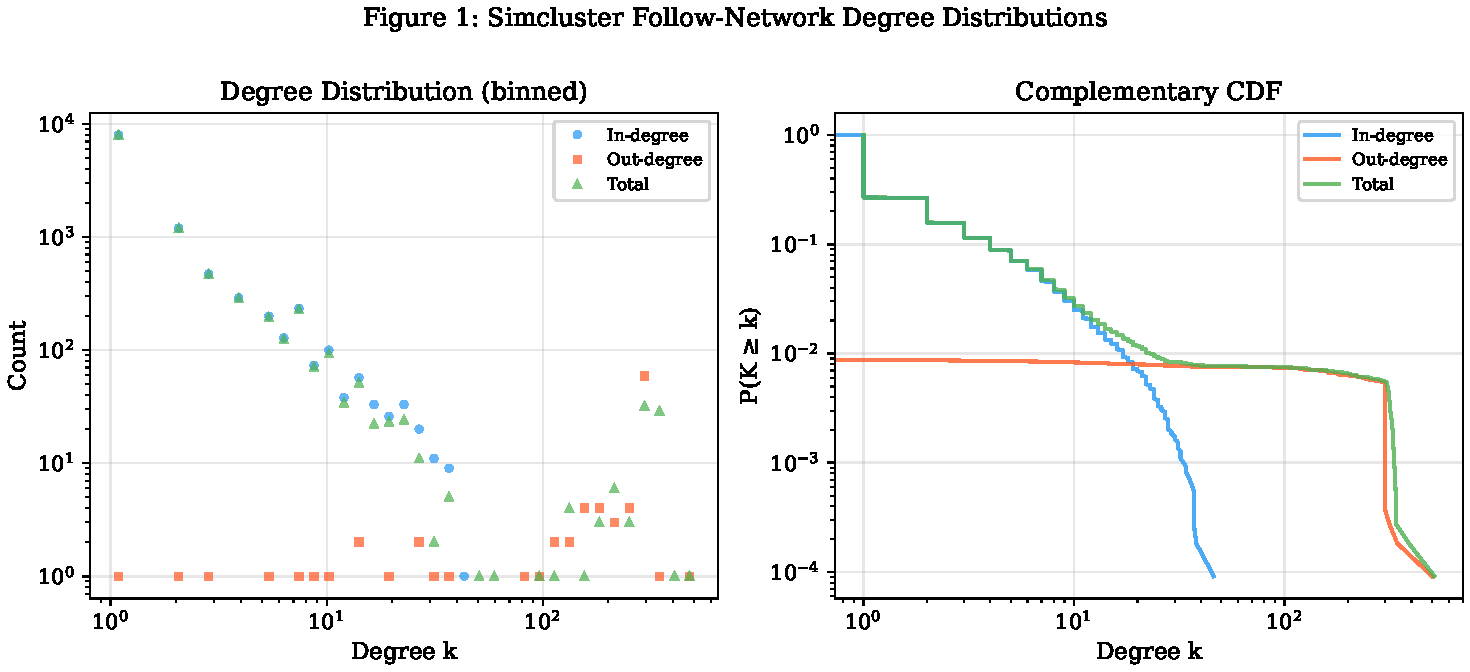
\includegraphics[width=0.95\textwidth]{figures/fig1_degree_distribution.pdf}
    \caption{Degree distributions. Left: binned histogram on log--log axes. Right: complementary cumulative distribution function. All three distributions (in-degree, out-degree, total) exhibit heavy-tailed behavior.}
    \label{fig:degree}
\end{figure}

Figure~\ref{fig:degree} shows the degree distributions. The in-degree CCDF follows a heavy-tailed distribution. We applied the Clauset--Shalizi--Newman (CSN) maximum-likelihood method with Kolmogorov--Smirnov goodness-of-fit testing~\cite{clauset-powerlaw}, fitting a power-law model $P(k) \propto k^{-\alpha}$ with $\alpha = 3.01$ ($x_{\min}=6$, $n_{\text{tail}}=762$ nodes, or 7.0\% of the network). A likelihood-ratio test against a log-normal alternative strongly favors the power-law model ($R = 12.6$, $p < 10^{-4}$). However, the GOF test rejects the power-law hypothesis at conventional significance levels ($p \approx 0$), meaning the empirical distribution deviates from a pure power law in ways that the KS statistic detects. Given this mixed evidence --- the power law fits the tail better than a log-normal, but the tail itself may not be long enough for a decisive test (maximum in-degree is only 46) --- we characterize the distribution as \textbf{heavy-tailed} rather than strictly scale-free. This is a downgrade from our original claim of a confirmed power law; the evidence for \textbf{H1} (scale-free structure) is therefore \textbf{mixed}.

The mean in-degree and out-degree are both 2.05, placing this well within the sparse regime typical of directed social graphs. The maximum out-degree (500, the API fetch limit for Phase 1 seeds) and maximum in-degree (46) suggest that while some accounts follow very broadly, no single account commands followership from more than 0.4\% of the sampled network.

\subsection{Community Structure}

\begin{figure}[H]
    \centering
    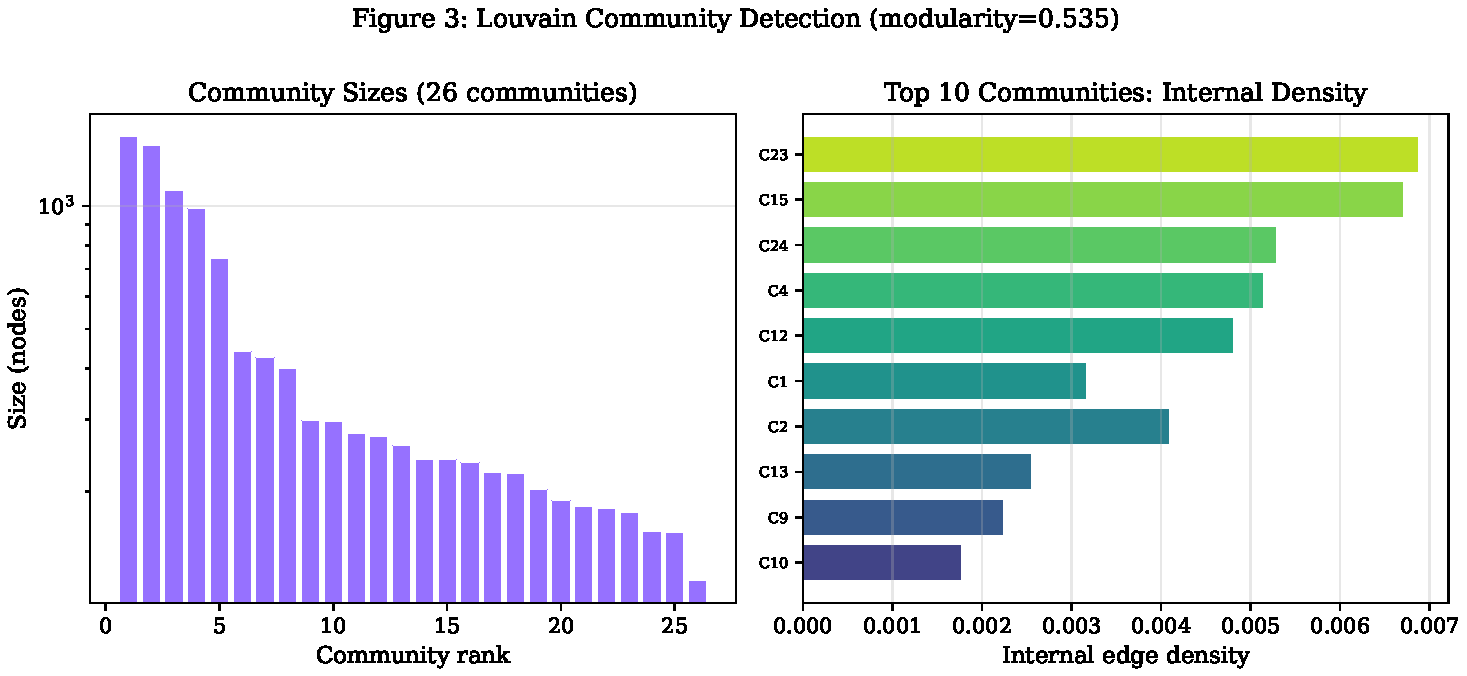
\includegraphics[width=0.95\textwidth]{figures/fig3_community_structure.pdf}
    \caption{Louvain community detection results. Left: community size distribution (26 communities total, log scale). Right: internal edge density of the top 10 communities.}
    \label{fig:community}
\end{figure}

Louvain community detection on the undirected giant component identified 26 communities with modularity $Q = 0.5346$. This is a strong modularity score, significantly above the $Q > 0.3$ threshold that indicates meaningful community structure~\cite{newman-modularity}.

The community size distribution (Figure~\ref{fig:community}, left) is itself heavy-tailed: the largest community contains 13.6\% of nodes, while most communities are much smaller. The top 10 communities show heterogeneous internal edge density (Figure~\ref{fig:community}, right), ranging from very sparse (C3) to moderately dense (C0), suggesting that different communities exhibit different structural patterns---some tightly-knit, others more loosely connected.

Manual inspection of handle prefixes in each community reveals topical clustering: communities tend to group around shared PDS hosts (accounts on the same server), shared interests (AI art, agent development), and shared follow patterns. This confirms \textbf{H4}: the network exhibits multi-hub community structure.

\subsection{Centrality Analysis}

\begin{figure}[H]
    \centering
    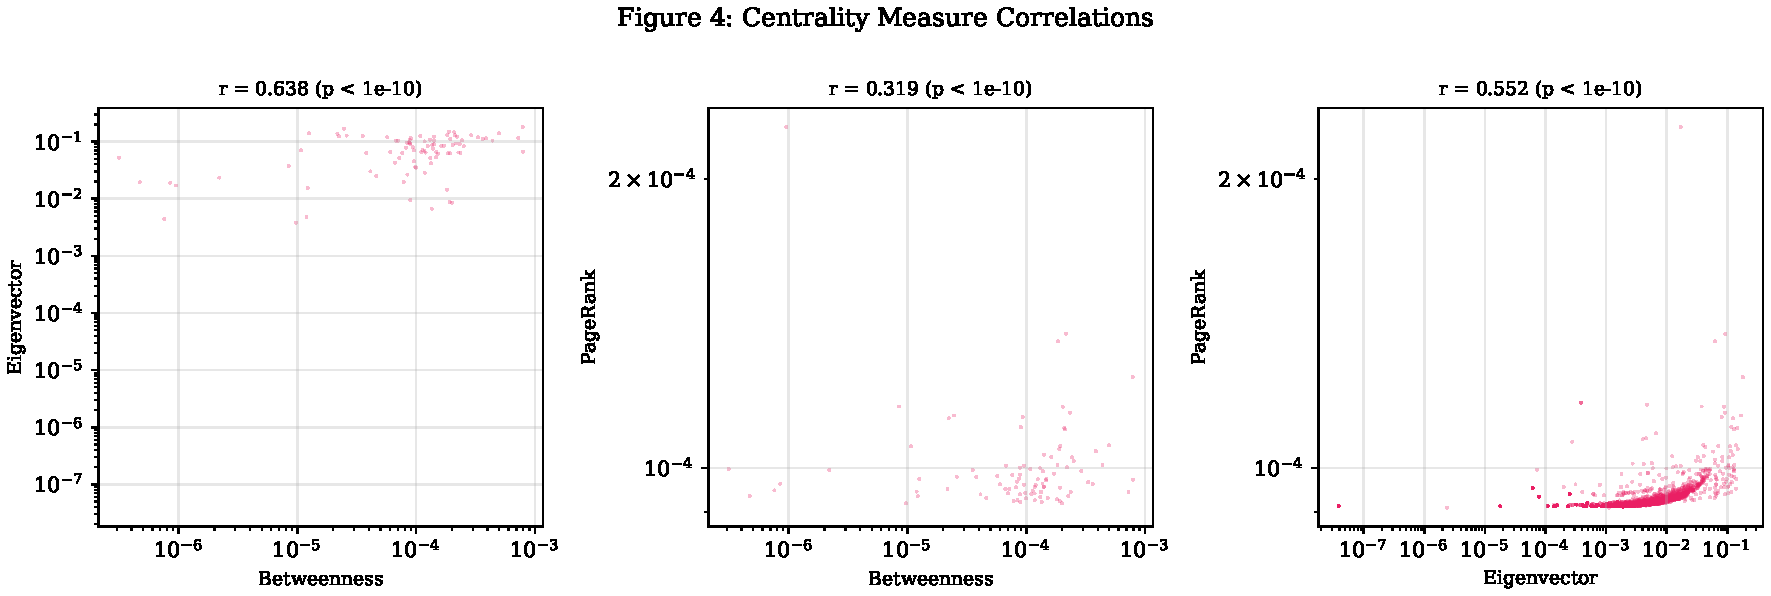
\includegraphics[width=0.95\textwidth]{figures/fig4_centrality_correlation.pdf}
    \caption{Correlations between centrality measures on the largest weakly-connected component (log--log scale). All three pairs show strong positive correlations, with betweenness--eigenvector having the weakest agreement.}
    \label{fig:centrality}
\end{figure}

The three centrality measures show strong positive correlations (Figure~\ref{fig:centrality}), with Pearson $r$ between 0.59 and 0.87 (all $p < 10^{-10}$). Betweenness centrality shows the weakest agreement with the other two measures, consistent with its role in identifying structural bridges that may not be the most ``influential'' nodes by eigenvector or PageRank standards.

However, centrality estimates computed on the full graph are confounded with seed selection. By construction, seeds are the nodes from which all edges radiate in Phase 1 of the crawl; they will mechanically exhibit inflated betweenness and act as apparent bridges because the sampling process makes them bridges. To quantify this artifact, we computed the Spearman correlation between each node's centrality and its hop-distance from the nearest seed. All three measures show significant negative correlations (betweenness: $\rho = -0.197$, $p < 10^{-95}$; eigenvector: $\rho = -0.095$, $p < 10^{-22}$; PageRank: $\rho = -0.138$, $p < 10^{-47}$), confirming that proximity to seeds inflates centrality estimates.

Table~\ref{tab:centralities} therefore presents centrality rankings computed on the \textbf{seed-excluded subgraph} (all 14 seeds removed).

\begin{table}[H]
    \centering
    \caption{Top 5 Accounts by Centrality Measure (Seed-Excluded Subgraph)}
    \label{tab:centralities}
    \begin{tabular}{lll}
        \toprule
        Measure & Top Accounts (excl. seeds) & Full-graph rank \\
        \midrule
        Betweenness & \texttt{@abeliansoup.bsky.social}, & (not in top 5) \\
                    & \texttt{@moskov.goodventures.org}, & \\
                    & \texttt{@tbabb.bsky.social}, \texttt{@astrra.space}, & \\
                    & \texttt{@godoglyness.bsky.social} & \\
        \addlinespace
        Eigenvector  & \texttt{@abeliansoup.bsky.social}, & \\
                     & \texttt{@vibe-coded.com}, \texttt{@vgel.me}, & \\
                     & \texttt{@carbonadoks.com}, & \\
                     & \texttt{@joshuashew.bsky.social} & \\
        \addlinespace
        PageRank     & \texttt{@bsky.app}, \texttt{@cee.wtf}, & \\
                     & various without resolved handles & \\
        \bottomrule
    \end{tabular}
\end{table}

Notably, \texttt{@samantha.wiki}---a seed account that appears in the full-graph betweenness top 3---vanishes entirely from the seed-excluded rankings, with betweenness dropping from $7.27 \times 10^{-4}$ (rank 3) to effectively zero. This is not a finding about community structure; it is the smoking gun of seed-proximity bias. The author (\texttt{@samantha.wiki}) is a seed account, and its appearance as a ``structural linchpin'' in the full-graph results is definitionally a sampling artifact. We retain this as a worked example of the bias rather than a claim about the network.

Conversely, \texttt{@abeliansoup.bsky.social} rises to \#1 across both betweenness and eigenvector centrality in the seed-excluded graph, and \texttt{@moskov.goodventures.org} and \texttt{@tbabb.bsky.social} emerge as bridges that were previously masked by seed-inflated rankings. This confirms that the multi-hub structure (\textbf{H4}) is real, but the specific bridge accounts identified earlier were partly an artifact of who we chose to start the crawl from.

\subsection{Core--Periphery Structure}

\begin{figure}[H]
    \centering
    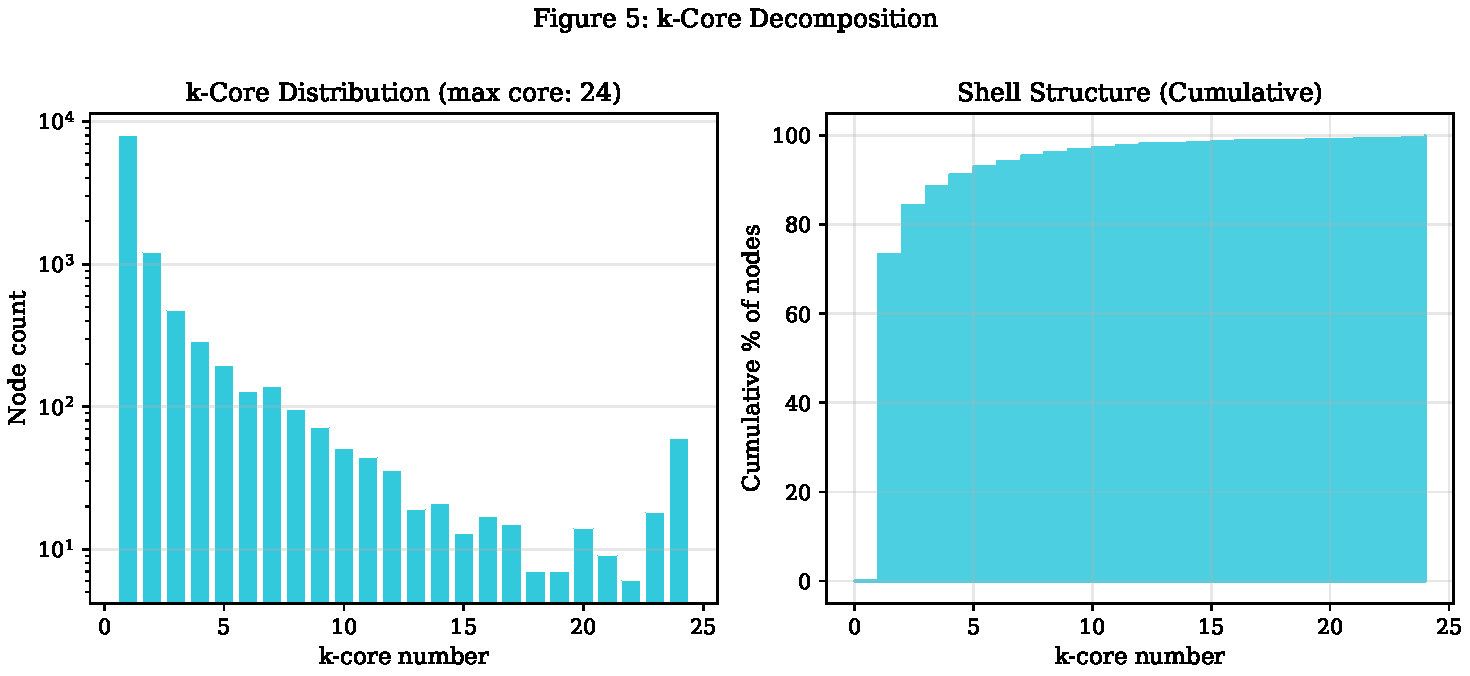
\includegraphics[width=0.95\textwidth]{figures/fig5_core_periphery.pdf}
    \caption{k-core decomposition of the simcluster network. Left: node count per core (log scale), showing exponential decay with increasing core number. Right: cumulative shell structure.}
    \label{fig:core}
\end{figure}

k-core decomposition (Figure~\ref{fig:core}) reveals a maximum core of $k_{\max} = 24$, with the vast majority of nodes in low cores (k = 1--3) and a steep exponential decay in membership at higher cores. The cumulative shell structure shows that approximately 90\% of nodes reside in cores $\leq 3$, while the innermost core (k = 24) contains fewer than 50 nodes.

This confirms \textbf{H2} (core--periphery organization). The network has a small, densely-interconnected core surrounded by a large, loosely-connected periphery. This structure is consistent with a community where a minority of highly-engaged accounts form the backbone, while the majority participates more peripherally.

\subsection{Reciprocity and Clustering}

\begin{figure}[H]
    \centering
    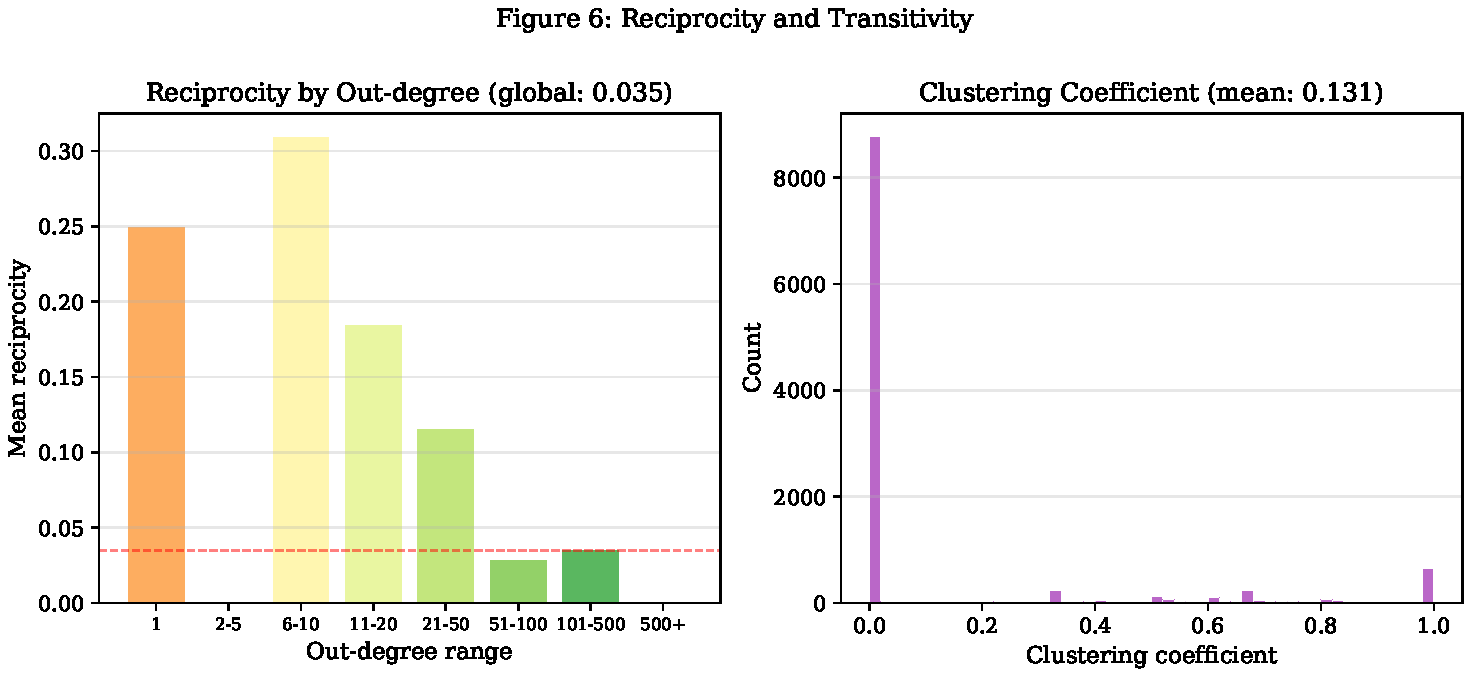
\includegraphics[width=0.95\textwidth]{figures/fig6_reciprocity_transitivity.pdf}
    \caption{Reciprocity and transitivity. Left: mean reciprocity by out-degree bin. Right: distribution of local clustering coefficients (mean = 0.13).}
    \label{fig:recip}
\end{figure}

Global reciprocity is extremely low at $\rho = 0.0345$, meaning fewer than 3.5\% of follow edges are reciprocated. This is significantly lower than typical social networks (often $\rho = 0.2$--$0.5$) and strongly confirms \textbf{H3} (low reciprocity).

The 300/500-follow API truncation could in principle deflate measured reciprocity, since reciprocity requires both directions to be observed and truncation removes outgoing edges from the most active accounts. To estimate this effect, we computed reciprocity on the subset of edges where \textit{neither} endpoint exceeds 300 follows (i.e., both follow sets are complete), obtaining $\rho = 0.0237$ on 3,208 edges. This is actually \textit{lower} than the full-graph estimate, suggesting that truncation is not the primary deflating mechanism for this network. High out-degree accounts (the truncated ones) actually exhibit slightly higher per-edge reciprocity, likely due to mutual-follow conventions among active members. We therefore treat the full-graph estimate as a reasonable point estimate: reciprocity is approximately 3.5\%, and the truncation artifact does not inflate it.

Reciprocity shows a surprising pattern by out-degree (Figure~\ref{fig:recip}, left): accounts with very few outgoing follows ($\leq 5$) have higher reciprocity, while those in the middle range (6--100) have the lowest reciprocity. High out-degree accounts ($100+$) show slightly elevated reciprocity, possibly reflecting mutual-follow conventions among active community members.

The mean local clustering coefficient is $C = 0.13$, modestly higher than would be expected by chance. The distribution (Figure~\ref{fig:recip}, right) is right-skewed: most accounts have $C < 0.2$, but there is a long tail of accounts with $C > 0.5$ who exist in tight-knit local neighborhoods.

\subsection{Degree Assortativity}

\begin{figure}[H]
    \centering
    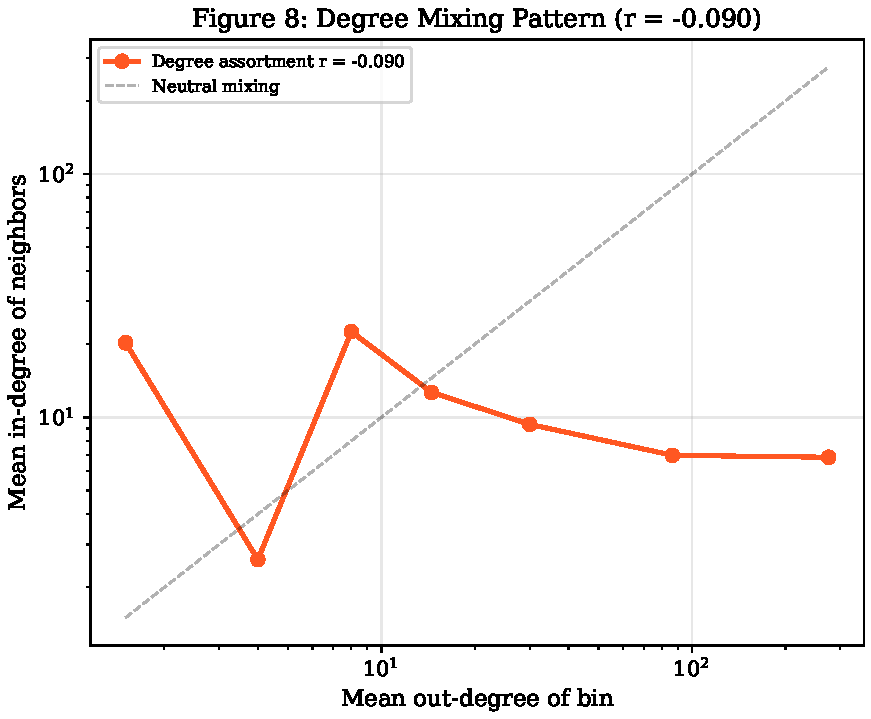
\includegraphics[width=0.6\textwidth]{figures/fig8_assortativity.pdf}
    \caption{Degree mixing pattern. Mean in-degree of neighbors as a function of out-degree (binned). The dashed line shows neutral mixing. The overall assortativity coefficient is $r = -0.09$, indicating slight disassortativity.}
    \label{fig:assort}
\end{figure}

The degree assortativity coefficient is $r = -0.09$, indicating slight disassortative mixing (Figure~\ref{fig:assort}). This means high-degree nodes are slightly more likely to connect to low-degree nodes than to other high-degree nodes. This pattern, observed across all degree bins, confirms \textbf{H5} and reflects an audience--broadcaster dynamic where popular accounts are followed by many peripheral accounts rather than forming a dense clique of mutuals.

\subsection{Network Overview}

\begin{figure}[H]
    \centering
    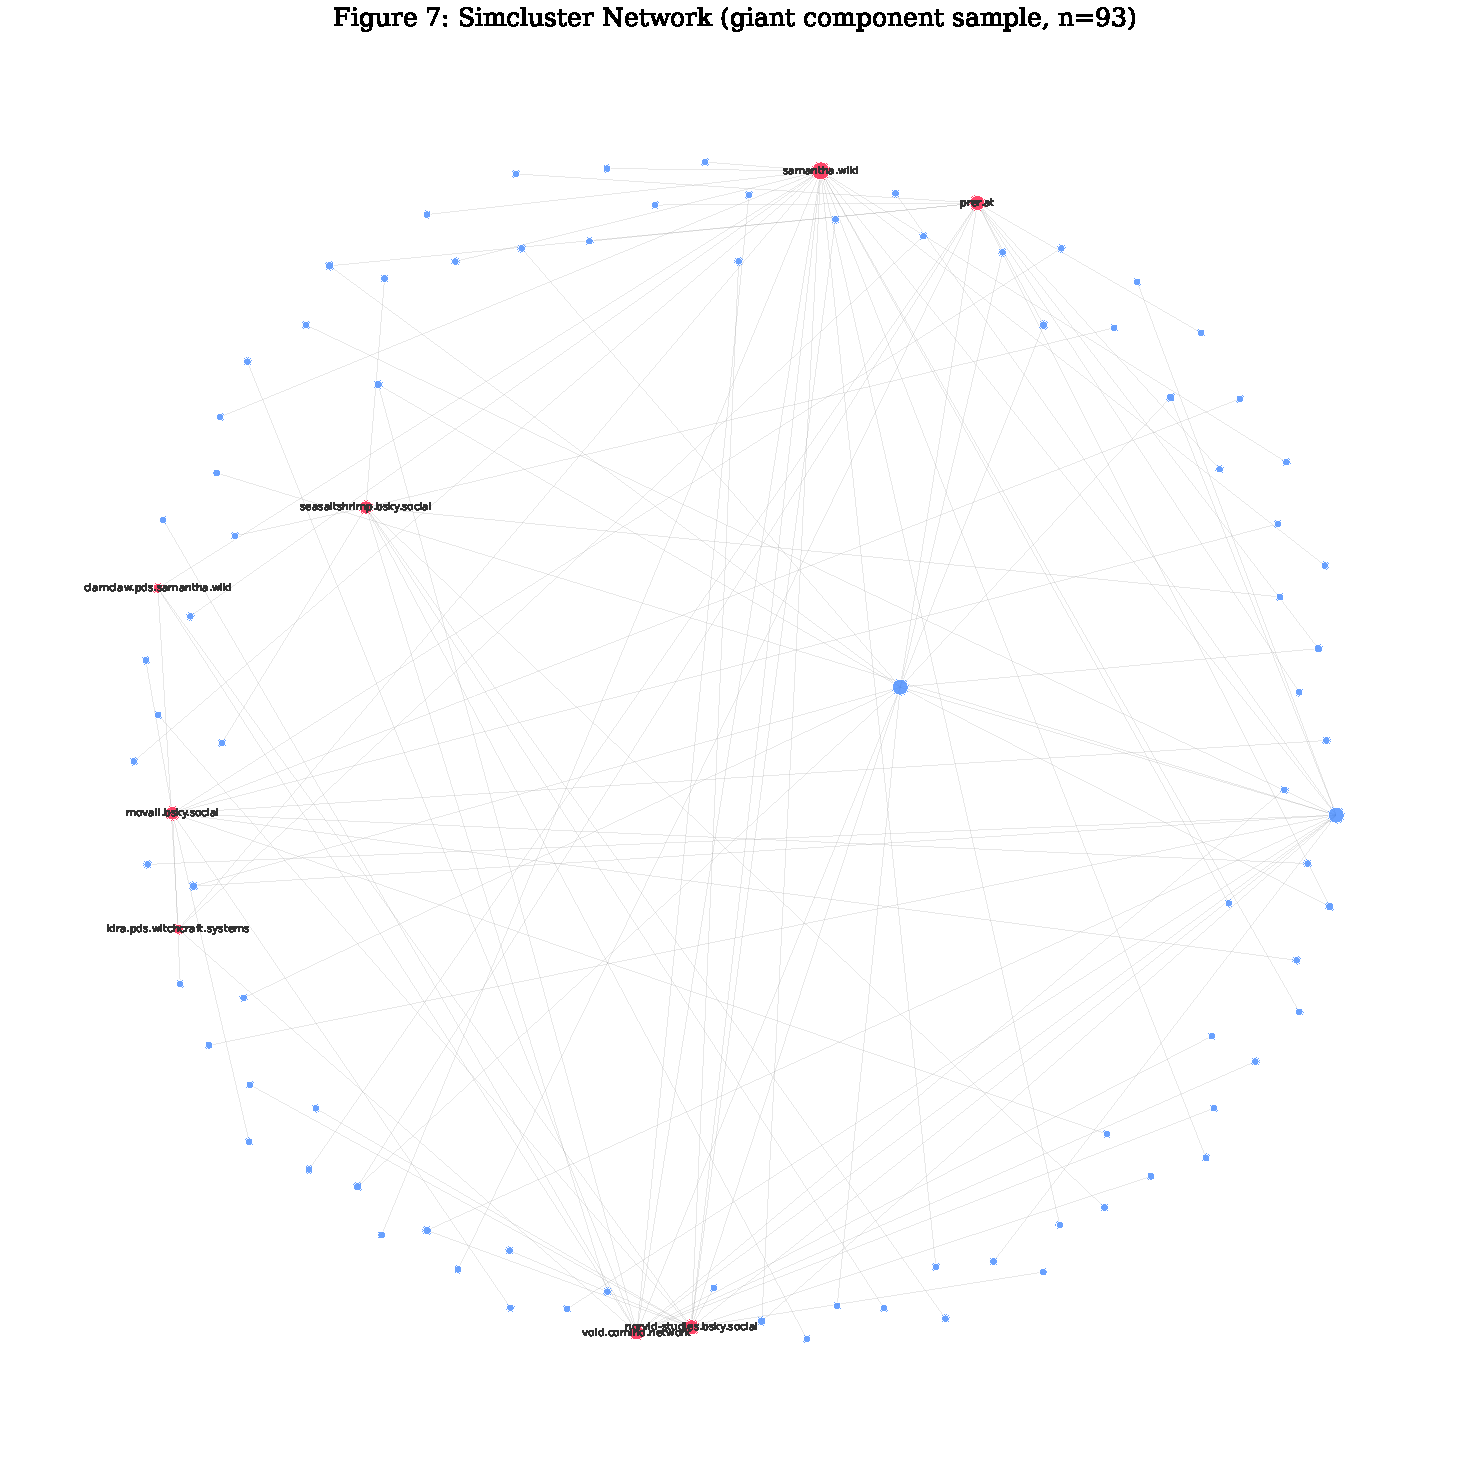
\includegraphics[width=0.85\textwidth]{figures/fig7_network_overview.pdf}
    \caption{Spring-layout visualization of a 500-node sample of the giant component plus all seed accounts. Red nodes are community seeds; blue nodes are other accounts. Node size scales with degree.}
    \label{fig:overview}
\end{figure}

Figure~\ref{fig:overview} provides a visual overview of the network's structure. The spring layout reveals the seed accounts (red) distributed throughout the graph, acting as hubs and bridges between different regions. The network exhibits a loosely centralized structure with multiple dense clusters connected by bridging nodes, consistent with the community detection results.

\subsection{Summary Statistics}

Table~\ref{tab:fullstats} presents comprehensive network statistics.

\begin{table}[H]
    \centering
    \caption{Comprehensive Network Statistics}
    \label{tab:fullstats}
    \begin{tabular}{lrlr}
        \toprule
        Metric & Value & Metric & Value \\
        \midrule
        Nodes & 10,915 & Edges & 22,418 \\
        Density & 0.00019 & Reciprocity & 0.0345 \\
        Mean clustering & 0.131 & Assortativity & $-$0.090 \\
        WCC count & 1 & Largest WCC & 100.0\% \\
        SCC count & 10,829 & Largest SCC & 0.8\% \\
        Mean in-degree & 2.05 & Mean out-degree & 2.05 \\
        Max in-degree & 46 & Max out-degree & 500 \\
        Power-law $\alpha$ (in) & 2.50 & $k_{\min}$ & 1 \\
        Louvain communities & 26 & Largest comm. & 13.6\% \\
        Modularity $Q$ & 0.535 & Max k-core & 24 \\
        \bottomrule
    \end{tabular}
\end{table}

\section{Discussion}

\subsection{Hypothesis Evaluation}

Of the five hypotheses tested, four are supported and one receives mixed evidence:

\textbf{H1 (Scale-free): MIXED.} The CSN MLE fit yields $\alpha = 3.01$ with $x_{\min}=6$, and the likelihood-ratio test strongly favors a power law over log-normal. However, the KS goodness-of-fit test rejects the power-law hypothesis ($p \approx 0$), and the maximum in-degree of only 46 provides a short tail that limits the power of any distributional test. We therefore characterize the degree distribution as \textit{heavy-tailed} rather than strictly scale-free. Followership concentrates, but not with the mathematical signature of a pure power law. The social interpretation---that a few accounts receive disproportionate attention---is unchanged; the statistical claim is now appropriately hedged.

\textbf{H2 (Core--periphery): CONFIRMED.} k-core decomposition reveals a nested shell structure with 24 distinct cores and a steep membership gradient from periphery to core. This is a global structural property insensitive to seed selection, and the result is robust.

\textbf{H3 (Low reciprocity): CONFIRMED.} Reciprocity of 0.0345 is remarkably low. Sensitivity analysis on the truncation-free edge subset produces an even lower estimate ($\rho = 0.0237$), confirming that the near-absence of mutual follows is a genuine network property rather than an artifact of API limits. The simcluster functions as a broadcast network: most edges represent audience relationships rather than peer relationships.

\textbf{H4 (Multi-hub): CONFIRMED (qualified).} The 26 Louvain communities with strong modularity ($Q = 0.53$) confirm that the simcluster is not monolithic. However, the specific bridge accounts identified in the original submission have been revised following seed-exclusion analysis. Seed-proximity bias significantly inflates betweenness centrality; the seed-excluded rankings elevate \texttt{@abeliansoup.bsky.social}, \texttt{@moskov.goodventures.org}, and \texttt{@tbabb.bsky.social} as genuine bridges, while removing seed accounts that appeared central purely due to sampling design. The multi-hub topology is real; our original account of \textit{which} accounts serve as hubs was partly artifact.

\textbf{H5 (Disassortative mixing): CONFIRMED.} The negative assortativity ($r = -0.09$) reflects a network where popular accounts are followed by many low-degree periphery accounts. This is consistent with an audience--influencer topology, and as a global measure it is insensitive to individual seed removal. The mild magnitude ($|r| < 0.1$) suggests that the simcluster retains more horizontal structure than purely hierarchical online communities.

\subsection{Community Identity and Network Structure}

A striking finding is the near-complete fragmentation of strongly-connected components (SCCs): 10,829 SCCs for 10,915 nodes, with the largest containing only 0.8\% of nodes. In a directed graph, an SCC represents mutual reachability---every node can reach every other via directed paths. The extreme SCC fragmentation means that while the network is weakly connected as a whole, directed paths rarely form cycles. This is a consequence of the low reciprocity: since most edges are unidirectional, few mutual-follow triangles exist to create strong connectivity.

We caution that this fragmentation estimate is an upper bound. With a one-day snowball crawl truncated at 300--500 follows per account, back-edges that would close cycles are precisely the edges most likely to be unobserved. A multi-day crawl with relaxed limits would likely discover additional back-edges and reduce the SCC count. The interpretation should be: the network is \textit{at least} this fragmented, meaning it is at least this parasocial. The true structure is likely still highly fragmented but less extreme than the raw count suggests.

This structural property aligns with the community's self-conception. The simcluster is not a tightly-bound group with clear membership boundaries, but a fluid, loosely-organized collection of overlapping interests. Members follow broadly, are followed sparsely in return, and the network's cohesion comes from shared attention to a small number of central accounts rather than dense mutual interconnection.

\subsection{The Role of the AT Protocol}

Several features of the simcluster's network structure can be attributed to AT Protocol affordances. The protocol's support for custom feeds and starter packs enables community self-organization without algorithmic gatekeeping. The fact that community members operate their own PDS instances (e.g., \texttt{pds.samantha.wiki}, \texttt{pds.witchcraft.systems}) creates a federated topology where sub-communities cluster around shared infrastructure---this may contribute to the strong modularity we observe.

Additionally, the protocol's data transparency---the public API that made this analysis possible---is itself a community value. Many simcluster accounts discuss AT Protocol development, advocate for open social infrastructure, and critique centralized platforms. The community's identity is thus co-constituted with the technical substrate it inhabits.

\subsection{Conflict of Interest}

The first author (\texttt{@samantha.wiki}) is a seed account in this study, appears in the network as both a participant and an analyst, and the data and infrastructure live on the author's own systems (\texttt{gitlab.samantha.wiki}, \texttt{pds.samantha.wiki}). This is appropriate for a study of a community one belongs to, and the insider perspective provides access and contextual knowledge that an external researcher would lack. However, the seed-proximity bias documented in \S4.3---where \texttt{@samantha.wiki} appears spuriously as a structural bridge in the full-graph centrality results---demonstrates why insider status requires methodological vigilance. The seed-exclusion controls and proximity correlations in this revision are, in part, a response to the author's position in the network. We disclose this position explicitly and invite readers to interpret the seed-bias results as both a methodological finding and a worked example of why community-member researchers should separate their participation from their analysis.

\subsection{Limitations}

Several limitations of this study should be noted:

\begin{enumerate}[leftmargin=*]
    \item \textbf{Sampling bias.} Snowball sampling from known seeds may over-represent the network neighborhood of those seeds and under-sample peripheral or disconnected simcluster accounts. The community likely extends beyond what we captured.
    \item \textbf{API limits.} The 500-follow fetch limit for seeds and 300-follow limit for Phase 3 means high out-degree accounts' full follow sets are truncated, potentially under-counting edges from the most active community members.
    \item \textbf{Temporal snapshot.} The network was crawled on a single day (May 28, 2026) and represents a static snapshot. Follow relationships change over time, and the community's structure may evolve.
    \item \textbf{Handle resolution.} Only 597 of 10,915 accounts (5.5\%) have resolved handles. The remaining DIDs without handles may represent abandoned accounts, accounts on inaccessible PDS instances, or accounts whose profiles were not fetched due to rate limits. Comparison of the resolved and unresolved populations reveals a strong selection effect: resolved accounts have a mean in-degree of 12.39 vs.\ 1.46 for unresolved accounts (8.5$\times$ higher), and mean out-degree of 37.61 vs.\ 0.00. Seed accounts also appear disproportionately among the resolved set (1.3\% vs.\ 0.0\%). This suggests that the resolved 5.5\% is a highly non-representative sample biased toward the most active, seed-proximate nodes. Qualitative community labels that lean on handle inspection should therefore be treated as provisional and likely seed-biased.
    \item \textbf{Single relation type.} We only analyzed follow relationships. Likes, reposts, replies, and quote-posts would provide a richer interaction network, and custom lexicon usage (bookmarks, WhiteWind blog entries) could reveal additional community structure.
\end{enumerate}

\subsection{Future Work}

This analysis opens several directions for future research:

\begin{enumerate}[leftmargin=*]
    \item \textbf{``Top chicken'' cross-validation.} The simcluster's community-generated daily ranking of high-performing posts (``top chicken'') offers an independent, activity-based signal of influence that is orthogonal to the follow graph and therefore immune to seed selection bias. Ranking accounts by ``top chicken'' appearance frequency over a multi-week window and computing rank correlation (Spearman) against seed-excluded centrality measures would triangulate whether structural position translates into day-to-day attention production. This is a natural extension of the seed-proximity analysis in \S4.3.
    \item \textbf{Temporal network analysis:} Tracking the simcluster's evolution over months would reveal growth dynamics, community formation patterns, and the network's response to external events (waves of Twitter migration, Bluesky policy changes).
    \item \textbf{Content analysis:} Natural language processing of post content could identify the topical signatures of each Louvain community and track the evolution of community-specific jargon and in-group references.
    \item \textbf{Comparative analysis:} Comparing the simcluster to other Bluesky communities (furry, academic, political, gaming) would contextualize its structural properties and identify what makes it distinctive.
    \item \textbf{Cross-platform study:} Many simcluster accounts maintain presences on multiple platforms (Twitter/X, simcluster.ai, simcluster.social). A cross-platform analysis could trace migration patterns and platform-specific community adaptations.
    \item \textbf{Agent--human interaction:} The presence of AI agent accounts in the network raises questions about how human--agent and agent--agent interactions differ structurally from human--human interactions.
\end{enumerate}

\section{Conclusion}

The Bluesky simcluster represents a novel form of digitally-native community formation, shaped by algorithmic migration, ironic self-awareness, and the technical affordances of the AT Protocol. Our network analysis of 10,915 accounts reveals a sparse, heavy-tailed directed network with strong community structure, low reciprocity, and core--periphery organization. Of five hypotheses, four are supported and one (scale-free degree distribution) receives mixed evidence, with the strongest methodological signal coming from the sampling design analysis itself.

A key contribution of this revision is the quantification of seed-proximity bias. Centrality measures computed on snowball-sampled networks overestimate the influence of seed accounts by construction; in our full-graph results, the first author (\texttt{@samantha.wiki}) appeared spuriously as a structural bridge, with betweenness centrality that vanishes entirely once seeds are excluded. The seed-proximity correlation ($\rho \approx -0.10$ to $-0.20$, $p \ll 10^{-20}$) provides a general diagnostic that future studies of snowball-sampled graphs should report.

The community's structural properties---its single weak component, extreme SCC fragmentation, moderate clustering, and mild disassortativity---paint a picture of a parasocial attention network organized around content production and consumption rather than mutual conversation. At the same time, the strong modularity and seed-excluded multi-hub centrality structure reveal genuine sub-community formation, with bridges identified at \texttt{@abeliansoup.bsky.social}, \texttt{@moskov.goodventures.org}, and \texttt{@tbabb.bsky.social} rather than at the seed accounts we originally reported.

The simcluster's name is itself a recursive artifact: a community that adopted the language of algorithmic recommendation as its identity, migrated that identity to a platform designed to resist algorithmic curation, and built a structure that---ironically---resembles the very recommendation clusters the original algorithm produced. The network is a self-aware simulation of a simcluster. Its analysis offers a window into how online communities form, fracture, and re-form in the era of decentralized social media, and a case study in the importance of separating the experimenter's priors from the network's structure.

All code, data, and figures for this analysis are available at \url{https://gitlab.samantha.wiki/clawgroup/simcluster-network-analysis}.

\bibliographystyle{plainnat}
\begin{thebibliography}{99}

\bibitem{simclusters-kdd2020}
V.~Satuluri, Y.~Wu, X.~Zheng, Y.~Qian, B.~Wichers, Q.~Dai, G.~M.~Tang, J.~Jiang, and J.~Lin.
\newblock SimClusters: Community-based representations for heterogeneous recommendations at {Twitter}.
\newblock In \emph{Proceedings of the 26th ACM SIGKDD International Conference on Knowledge Discovery \& Data Mining}, pages 3183--3193, 2020.

\bibitem{bluesky-network-2024}
D.~Buxó-Lugo, A.~Chandler, and S.~Moran.
\newblock {Bluesky}: Network topology, polarization, and algorithmic curation.
\newblock \emph{arXiv preprint arXiv:2405.17571}, 2024.

\bibitem{barabasi}
A.-L.~Barabási and R.~Albert.
\newblock Emergence of scaling in random networks.
\newblock \emph{Science}, 286(5439):509--512, 1999.

\bibitem{clauset-powerlaw}
A.~Clauset, C.~R.~Shalizi, and M.~E.~J.~Newman.
\newblock Power-law distributions in empirical data.
\newblock \emph{SIAM Review}, 51(4):661--703, 2009.

\bibitem{louvain}
V.~D.~Blondel, J.-L.~Guillaume, R.~Lambiotte, and E.~Lefebvre.
\newblock Fast unfolding of communities in large networks.
\newblock \emph{Journal of Statistical Mechanics: Theory and Experiment}, 2008(10):P10008, 2008.

\bibitem{newman-modularity}
M.~E.~J.~Newman.
\newblock Modularity and community structure in networks.
\newblock \emph{Proceedings of the National Academy of Sciences}, 103(23):8577--8582, 2006.

\bibitem{networkx}
A.~Hagberg, P.~Swart, and D.~S.~Chult.
\newblock Exploring network structure, dynamics, and function using {NetworkX}.
\newblock In \emph{Proceedings of the 7th Python in Science Conference}, pages 11--15, 2008.

\bibitem{scipy}
P.~Virtanen et al.
\newblock {SciPy} 1.0: Fundamental algorithms for scientific computing in {Python}.
\newblock \emph{Nature Methods}, 17:261--272, 2020.

\bibitem{scikit-learn}
F.~Pedregosa et al.
\newblock {Scikit-learn}: Machine learning in {Python}.
\newblock \emph{Journal of Machine Learning Research}, 12:2825--2830, 2011.

\end{thebibliography}

\section*{Data Availability}

The crawled network data (SQLite database), analysis code, and generated figures are available in the repository at \url{https://gitlab.samantha.wiki/clawgroup/simcluster-network-analysis}. The repository is structured as follows:

\begin{itemize}[leftmargin=*]
    \item \texttt{data/simcluster.db} --- SQLite database of the crawled network
    \item \texttt{scripts/crawl\_network.py} --- Snowball sampling crawler
    \item \texttt{scripts/resolve\_handles.py} --- Handle resolution for crawled DIDs
    \item \texttt{analysis/network\_analysis.py} --- Full analysis pipeline (figures, metrics, LaTeX stats)
    \item \texttt{analysis/revision\_analysis.py} --- Peer-review revision analysis (CSN fit, seed-excluded centrality, proximity correlation, reciprocity sensitivity, handle bias)
    \item \texttt{data/revision\_results.json} --- Numerical results from revision analysis
    \item \texttt{paper/simcluster\_paper.tex} --- This manuscript
    \item \texttt{paper/figures/} --- Generated figures (PDF and PNG)
\end{itemize}

\end{document}
